
Sur le green d'un golf, le contrat est assez simple. Il faut mettre la balle dans le trou. Si le putter tape la balle bien perpendiculairement à la trajectoire sur un green plat, la balle tombe dans le trou.


\definecolor{xdxdff}{rgb}{0.49019607843137253,0.49019607843137253,1.}
\definecolor{ududff}{rgb}{0.30196078431372547,0.30196078431372547,1.}
\begin{tikzpicture}[line cap=round,line join=round,>=triangle 45,x=1.0cm,y=1.0cm]
\clip(-2.8,1.24) rectangle (5.08,3.96);
\draw [line width=2.pt] (3.16,2.46) circle (0.6381222453417527cm);
\draw [line width=5.2pt] (-2.28,3.26)-- (-2.28,1.78);
\draw [->,line width=2.pt] (-2.28,2.54) -- (1.24,2.52);
\begin{scriptsize}
\draw [fill=ududff] (-1.74,2.54) circle (2.5pt);
\draw[color=ududff] (-1.6,2.91) node {$B$};
\draw [fill=ududff] (3.16,2.46) circle (0.5pt);
\draw[color=ududff] (3.3,2.67) node {$T$};
\end{scriptsize}
\end{tikzpicture}

Mais, si le putter n'arrive pas bien perpendiculairement, la balle dévie et ne rentre pas dans le trou.


\definecolor{ududff}{rgb}{0.30196078431372547,0.30196078431372547,1.}
\begin{tikzpicture}[line cap=round,line join=round,>=triangle 45,x=1.0cm,y=1.0cm]
\clip(-3.,1.32) rectangle (4.12,4.);
\draw [line width=2.pt] (3.16,2.46) circle (0.6381222453417527cm);
\draw [line width=5.2pt] (-2.28,3.26)-- (-2.48,1.8);
\draw [->,line width=2.pt] (-2.28,2.54) -- (2.24,1.9);
\draw [line width=1.6pt,dash pattern=on 1pt off 1pt] (-2.28,2.54)-- (3.16,2.46);
\begin{scriptsize}
\draw [fill=ududff] (-1.72,2.46) circle (2.5pt);
\draw[color=ududff] (-1.58,2.83) node {$B$};
\draw [fill=ududff] (3.16,2.46) circle (0.5pt);
\draw[color=ududff] (3.3,2.67) node {$T$};
\draw [fill=black] (-2.28,3.26) circle (0.5pt);
\end{scriptsize}
\end{tikzpicture}


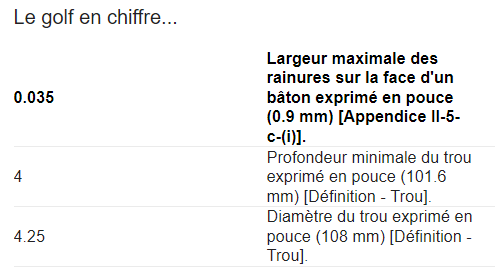
\includegraphics[scale=0.6]{TR-215.png} 


On considère que la balle touche le sol en un seul point. A 5 mètres du trou, quel est l'angle de déviation maximum pour que ma balle rentre dans le trou ?